\chapter{Literature Review}

This chapter presents a review of the literature surrounding memory latency reduction. It first focuses on more traditional methods, considering caching and then other methods of controlling latency, such as prefetching or scheduling. In the second section the focus moves to newer techniques that involve tracing and then finishes with a summary and evaluation of the position the literature presents. To place this review in context consider program running on a CPU with a Von Neumann architecture. This CPU has a single on-chip direct-mapped cache and connects to a memory system by way of an interconnect with other peripherals. This can be seen in Figure \ref{fig:journey-memory-transaction}.

Based on Figure \ref{fig:journey-memory-transaction}, if we consider a memory transaction from the processor that misses in the cache then where are the sources of latency and how large are they? The processor itself provides negligible latency, there is of course usually a delay between the instruction being fetched and decoded, but this would be incurred by any instruction so is not relevant to this discussion. Following that, there will be a cache miss in the internal cache so this will add latency, and then the control signals will cross into the system interconnect en-route to the memory controller and external memory, adding further latency. Once the control signals reach the memory controller main memory can be accessed, by far the biggest source of latency in this process. The data fetch can then be fed back up the system, is stored in the cache and is accessible to the processor adding further latency as it makes the return trip. 

\begin{figure}[ht]
	\tikzstyle{block} = [draw, rectangle, text width=2cm, text centered, minimum height=1.2cm, node distance=2.7cm,fill=blue!30]
\tikzstyle{container} = [draw, rectangle, inner sep=0.3cm, fill=orange!50,minimum height=3cm, minimum width=3cm]
\def\bottom#1#2{\hbox{\vbox to #1{\vfill\hbox{#2}}}}
\tikzset{
	mybackground/.style={execute at end picture={
			\begin{scope}[on background layer]
				\node[] at (current bounding box.north){\bottom{1cm} #1};
			\end{scope}
	}},
}
\begin{center}
	\begin{tikzpicture}
	
	    \node [block] (CPU) {CPU};
	    \node [block, below of=CPU] (cache) {L1 Cache};
	    \node [block, below of=cache, minimum width=5cm] (interconnect) {Interconnect};
	    \node [block, below of=interconnect,  minimum width=7cm, text width=7cm] (main) {Main Memory};
	    \begin{scope}[on background layer]
	    \node [container,fit=(CPU) (cache),label=above:CPU Die] (container) {};
		\end{scope}
	    \draw [thick] [->] ([xshift=2em]CPU.south)-- node[left] {\circled{1}} ([xshift=2em]cache.north);
	    \draw [thick] [->] ([xshift=-2em]cache.north)-- node[left] {\circled{6}} ([xshift=-2em]CPU.south);
	    \draw [thick] [->] ([xshift=2em]cache.south) -- node[left] {\circled{2}} ([xshift=2em]interconnect.north);
	    \draw [thick] [->] ([xshift=-2em]interconnect.north) -- node[left] {\circled{5}} ([xshift=-2em]cache.south);
	    \draw [thick] [->] ([xshift=2em]interconnect.south) -- node[left] {\circled{3}} ([xshift=2em]main.north);
	    \draw [thick] [->] ([xshift=-2em]main.north) -- node[left] {\circled{4}} ([xshift=-2em]interconnect.south);
	    
	    
	
	\end{tikzpicture}
\end{center}

	\caption[The Journey of a Memory Transaction]{A memory transaction follows a number of steps to satisfy a \gls{cpu} memory request. First in Step \circled{1} the \gls{cpu} issues a request to L1 cache to check for the presence of the memory element required. Suppose there is a cache miss then in Step \circled{2} the cache signals to the \gls{cpu} that there has been a cache miss and so the \gls{cpu} sends a signal via the interconnect, which then in Step \circled{3} signals main memory to get the data required. In Step \circled{4} and \circled{5} this data is passed back to the L1 Cache which stores it and then passes it to the \gls{cpu} in Step \circled{6}.}
	\label{fig:journey-memory-transaction}
\end{figure}

Having seen the journey of a memory transaction we have 3 sites that could be focussed on to reduce latency: the cache, the memory controller or the memory hardware. In this review we will not consider the memory hardware, despite it being the largest source of latency. This is because, as \citet{pattersonComputerOrganizationDesign2018} describe, choosing a memory technology is a trade-off between speed and cost, with the general principle being that faster memory is more expensive per unit. In my review of the literature I have found no papers that are proposing to have resolved this trade-off. All are proposing improvements to existing technologies, or new ones that fit into the existing cost/speed model. If we want to make a real difference to latency, we have to look elsewhere, accepting that main memory will always be slow relative to the processor, no matter how much we improve on its design.

On a final note before we begin, due to this literature review covering a broad range of topics, and most to quite a high depth, the digram presented in Figure \ref{fig:lit-review-schematic} maps out the various topics and their relationship to each other. Reading the review in concert with this diagram can help to locate yourself within the research presented and see the relationships between the topics included as they are presented.

\begin{sidewaysfigure}
	\begin{forest}
[{Memory Latency Reduction Techniques}
		[{Cache Intrinsic Techniques}
			[{Replacement Policy}
				[{Arrival Time Based}]
				[{Frequency Based}]
				[{Recency Based}] 
				[{Combined Recency \& Frequency}]
				[Fusion]
			]
			[{Cache Architectures}
				[{Increased Associativity}] 
			]
		]	
		[{Cache Extrinsic}]
		[Tracing]
]  
\end{forest}
	\caption[Literature Review Structure]{The structure of the Literature Review showing the topics and subtopics covered, organised into sections. The review is conducted via a depth-first search of these topics.}
	\label{fig:lit-review-schematic}
\end{sidewaysfigure}

\section{Cache Intrinsic Techniques}

\label{sec:cache}

After their first introduction to super-computers in the 1960's \cite{pattersonComputerOrganizationDesign2018} caches have become a standard part of almost any memory architecture. Iterative improvements, thanks to Moore's law, have pushed the performance of caches to higher and higher levels, hiding more and more latency as their information density increases. Despite advances in technology, it is still the case that the cache replacement policy is the most significant factor in determining how effective a cache will be at reducing memory latency \cite{hennessyComputerArchitectureQuantitative2019}.

\subsection{Cache Replacement Policy}
\label{sec:replacement_policy}

In its simplest form a cache replacement policy is simply a way of deciding which cache line is replaced when a cache reaches capacity. For direct-mapped caches they are not important, but in set-associative caches the choice of replacement policy is absolutely crucial \cite{hennessyComputerArchitectureQuantitative2019}, and there has been much research into which policies yield the best outcomes across a variety of metrics\footnote{In this discussion of cache policies reducing miss rate and reducing latency can be thought of as synonymous, due to cache misses being the main source of latency.}.

When discussing various policies that are useful in reducing latency it's good to have in mind two policies that are often referred to in the literature but are not actually implemented. The first of these is known as \texttt{OPT} or \texttt{MIN} \cite{jeongOptimalReplacementsCaches1999} a theoretical optimal replacement policy, which can perfectly predict which cache block will be needed furthest in the future. This means \texttt{OPT} will provably suffer the lowest number of cache misses of any cache policy. The second theoretical replacement policy is that of random replacement or \texttt{RAND}. Under this scheme when a decision on replacement has to be made, the choice is made completely at random without reference to any other information \cite{beladyStudyReplacementAlgorithms1966}. Again this method is not usually implemented by cache designers when optimising for latency reduction \cite{karedlaCachingStrategiesImprove1994} but its utility is as the lower extreme of a continuum, bounded by \texttt{OPT} at the other extreme. allowing policy designers to empirically assess new policies in relation to \texttt{OPT} and \texttt{RAND}.

\subsubsection{Arrival-Time Based Techniques}

One of the more simple cache replacement policies is to decide which cache line is to be replaced based on when the cache line entered the cache. This is known as the cache line's arrival time. The most common formulation of this is a policy that removes the item inserted furthest back in the past, implemented using a FIFO queue.

A lot of implementers choose this technique because it has a very low hardware requirement \cite{pandaSurveyReplacementStrategies2016} which leads to a low cost. On the other hand it's not highly performative at reducing latency \cite{al-zoubiPerformanceEvaluationCache2004, tsaoMultiFactorPagingExperiment1972}, often performing similarly to \texttt{RAND} despite the slight increase in hardware. \gls{fifo} is also susceptible to Belady's Anomaly \cite{beladyAnomalySpacetimeCharacteristics1969} so there's no guarantee that larger caches will produce lower miss rates. Due to its low performance, research into using \gls{fifo} queues has been limited, with \gls{fifo} being used a baseline \cite{faresPerformanceEvaluationTraditional2012} rather than being implemented in its own right.

However some work has been done to improve \gls{fifo}. \citet{turnerSegmentedFIFOPage1981} develop the idea of \gls{sfifo}, which partitions main memory into two sections. This creates a pseudo multi-level cache (see Section \ref{sec:multi-level}) but at a lower hardware cost. In the same vein, \citet{devilleLowcostUsagebasedReplacement1990} augments \gls{fifo} with a usage counter per set to do the partitioning in a more granular way. In more recent times \citet{wei-chetsengPRRLowoverheadCache2012} have experimented with combining a \gls{fifo} policy with cache-line locking. All these policies perform comparably to \gls{lru} (see Section \ref{sec:recency}) and use less hardware to do so. All in all \gls{fifo} is a good baseline to build from, and a viable option to implement if resources are limited, however we can use more information to make better decisions if we consider frequency of access. 

\subsubsection{Frequency Based Techniques}

A slightly more sophisticated approach to cache replacement is to count the number of times a cache block or line has been accessed, and then to evict the one with the lowest frequency of access. This approach is known as \gls{lfu}. In terms of implementation the most common form is to turn the cache into a priority queue where keys are calculated according to a variety of formula \cite{podlipnigSurveyWebCache2003}. In addition implementations choose between perfect \gls{lfu}, where every object is uniquely tracked across replacements, and in-cache \gls{lfu} where counts are only tracked when items are in the cache, though the latter option is most common \cite{podlipnigSurveyWebCache2003}.

Despite it's simplicity in concept, standard \gls{lfu} has several problems. The first is cache pollution \cite{karedlaCachingStrategiesImprove1994} where a cache block has a high number of accesses very early on and then is never referenced again. Having built up a high frequency count, the block stays in the cache for a long time, reducing its capacity. The second problem is that often you can end up with many different cache blocks having the same frequency count so you need some kind of tie-breaking arbitration \cite{podlipnigSurveyWebCache2003}.  Moreover, the hardware to keep track of all the frequency counts, potentially across multiple replacements, gives a very high hardware overhead and increased energy consumption \cite{pandaSurveyReplacementStrategies2016}. 

Some have attempted to address the shortcomings of \gls{lfu} with a variety of augmentations, most of which relate to adding ageing parameters to counter cache pollution. \citet{arlittEvaluatingContentManagement2000} suggests calculating the keys ($K_i$) in the priority queue that powers \gls{lfu} with a formula $K_i = C_i * F_i + L$. In this formulation $C_i$ is the cost of bringing an object into the cache, $F_i$ is the frequency that \gls{lfu} tracks and $L$ is equal to $K_f$ where $f$ is the most recently evicted cache element. He dubs this policy, \gls{lfuda}. Others like \citet{robinsonDataCacheManagement1990} choose to age slightly differently by protecting new entries to the cache and ageing the entire cache by reducing all reference counts $C$ to $\ceil[\big]{\frac{C}{2}}$ whenever the average reference count exceeds a predefined maximum value. Both of these techniques produce results comparable to \gls{lru} but the hardware cost is much higher due to the number of counters. In addition both of these approaches are concerned with the size of objects in the cache, something that is not a concern in this work.

A further augmentation of \gls{lfu} from \citet{kellyVariableQosShared1999} allows weighting parameters that come from the memory system to indicate how `useful' the caching of that element is. The problem, as \citeauthor{kellyVariableQosShared1999} admits, is the difficult of obtaining those weights and also the problem that this approach still requires the implementation of \gls{lru} as well to resolve ties. A final interesting approach to frequency type statistics is from \citet{mekhielMultiLevelCacheMost29} who proposes a two level cache with the \gls{mfu} elements going in the equivalent of an L1 cache and the \gls{lfu} elements going in an L2 cache. This allows frequently accessed data to be easily available to the \gls{cpu} and not easily evicted. This still suffers from the same cache pollution problems as other \gls{lfu} methods and still requires large amounts of hardware.

A slightly different approach is to take inspiration from probability theory as \gls{lfu-k} \cite{sokolinskyLFUKEffectiveBuffer2004} does, to predict the number of occurrences of an element (page, cache block etc.) in a reference string. The development from \gls{lfu} is that it adds extra terms into the estimation formula to account for the changing probability of referencing an element as time goes on. In this work \citeauthor{sokolinskyLFUKEffectiveBuffer2004} demonstrates that in terms of reducing cache miss rate, \gls{lfu-k} outperforms \gls{lfu} and \gls{lru}. However the effectiveness of this technique is intrinsically linked to the estimation of two parameters $m$ and $h$ neither of which is a trivial task. In addition the hardware requirements are still large, larger than \gls{lfu} due to the extra costs in calculating the probability functions. 

\gls{lfu} is an improvement from simple \gls{fifo} policies but suffers from the problem of cache pollution and a very high hardware requirement, particularly in the perfect case \cite{podlipnigSurveyWebCache2003}. Considering recency rather than frequency has long been considered a better metric to approximate how far in the future a piece of data will be needed, so the next section covers techniques that consider recency rather than frequency. 

\subsubsection{Recency Based Techniques}
\label{sec:recency}

Recency, as a general class of algorithms orders the elements in a cache by the time they were last referenced. This leads to two very general categories of recency-based algorithms, \gls{mrre} and \gls{lrre}. \gls{mrre} algorithms are much less common than \gls{lrre} and in general are less performant due to their poor temporal locality \cite{pandaSurveyReplacementStrategies2016}. As such we will not be focus on them in this thesis. The most popular \gls{lrre} algorithm is \gls{lru} \cite{pitkowSimpleRobustCaching1994, karedlaCachingStrategiesImprove1994, smithCacheMemories1982}. It makes use of temporal locality and, given a few simplifying assumptions, is very easy to implement.

However \gls{lru} is not without its problems. It performs very badly in a shared data environment, or when using virtual memory \cite{bansalCARClockAdaptive2004}. In addition, when the working set\footnote{See \cite{denningWorkingSetModel1968}} of the program exceeds the size of the cache, cache-thrashing \cite{denningThrashingItsCauses1968} occurs. This is most commonly seen in large loops \cite{linPredictingLastTouchReferences2002}. There's also the problem of dead blocks \cite{liuCacheBurstsNew2008}, where blocks read into memory are never referenced again but take time to be evicted, clogging up the cache. Finally, as \citet{linPredictingLastTouchReferences2002} describe, \gls{lru} does not have the desirable property that as associativity in the cache increases the miss rate decreases, the opposite is often true.

\paragraph{Statistical Inference}

Due to these shortcomings the important aspects of \gls{lru} from our point of view are the extensions of \gls{lru} to overcome them. The first of these is to try and use statistical inference or measured history of accesses to divine the future behaviour of a program and act accordingly. This is the approach taken by \citet{oneilLRUKPageReplacement1993} where the \gls{lru-k} algorithm is described. This technique uses Bayesian methods to estimate the inter-arrival times of memory references from the collected set of past references. \citet{vakaliLRUbasedAlgorithmsWeb2000} continues this idea with the \gls{hlru} policy. Under this scheme a function $hist(x,h)$ is defined which returns the $h$\textsuperscript{th} past reference to the cache object $x$, and then uses the maximum value of $hist$ among the cached objects to decide a replacement.

\citet{wongModifiedLRUPolicies2000} describe a suite of algorithms that are improvements of each other \gls{prl} and \gls{orl}. The essential idea of these algorithms is to favour lines that exhibit temporal behaviour by marking them using special instructions. \gls{prl} does the identification offline using profiling but \gls{orl} does profiling at run-time, keeping a table of hits to non-\gls{mru} lines and using this to set temporal bits. All of these policies show increased performance over \gls{lru} to varying degrees, but the problem with all of them is the extra hardware and book-keeping required. In addition none of these algorithms address some of the underlying flaws in \gls{lru} such as its susceptibility to flooding \cite{glassAdaptivePageReplacement1997}. The next set of approaches address these concerns.

\paragraph{Overcoming Flooding}

\begin{figure}[ht]
	\tikzset{
	print/.style={ % requires library shapes.symbols
		draw,
		tape,
		tape bend top=none
	}
}

\tikzstyle{block} = [draw, rectangle, text width=2cm, text centered, minimum height=1.2cm, node distance=2.7cm,fill=blue!30]
\tikzstyle{cache} = [rectangle split, rectangle split parts=4, draw, minimum width=2.5cm,font=\small, rectangle split part align={center}, fill=blue!30]


\begin{center}	
	\begin{tikzpicture}
	
		\node [print, fill=yellow!30] (assembly-code) {\lstinputlisting[language=risc-v, basicstyle=\ttfamily, numbers=left]{diagrams/flooding.S}};
	
		\node [cache, right=1cm of assembly-code, yshift=3.3cm] (iteration1)
		{             
			\textbf{Cache - First Iteration - Line 10}
			\nodepart{two} \texttt{0x4512} - (Addr: \texttt{0x2000})
			\nodepart{three} \texttt{0x2378} - (Addr: \texttt{0x2004})
			\nodepart{four} \texttt{0x9174} - (Addr: \texttt{0x2008})
		};
	
		\node[cache, below=of iteration1] (iteration2)
		{             
			\textbf{Cache - Second Iteration - Line 7}
			\nodepart{two} \texttt{0x7170} - (Addr: \texttt{0x200c})
			\nodepart{three} \texttt{0x2378} - (Addr: \texttt{0x2004})
			\nodepart{four} \texttt{0x9174} - (Addr: \texttt{0x2008})
		};
	
		\node[cache, below=of iteration2] (iteration3)
		{             
			\textbf{Cache - Second Iteration - Line 8}
			\nodepart{two} \texttt{0x7170} - (Addr: \texttt{0x200c})
			\nodepart{three} \texttt{0x4512} - (Addr: \texttt{0x2000})
			\nodepart{four} \texttt{0x9174} - (Addr: \texttt{0x2008})
		};
		
	\end{tikzpicture}
\end{center}
	\caption[Flooding Example]{Flooding usually occurs in large loops, where the working set of the program exceeds the size of the cache. The example above demonstrates this. On the first three loads of the first iteration everything proceeds as usual. Once Line 10 is hit however the element from address \texttt{0x2000} is evicted under the \gls{lru} policy leading to the situation we see in the second example cache above. Then when Line 7 executes in the second iteration we are forced to evict the element from address \texttt{0x2004}. Consequently the cache is useless in this situation as it every memory access will be a miss, this is flooding.}
	\label{fig:flooding}
\end{figure}

Flooding is a phenomenon particularly associated with \gls{lru} which happens when applications try to access a large address space in a sequential fashion. As more addresses are accessed and the cache capacity is exhausted, old elements (those at the beginning of the space) are evicted from the cache, and then when the loop begins again old elements are pushed out, this is shown in Figure \ref{fig:flooding}. This means that the cache policy has no positive impact on the execution at all. To address this \citet{glassAdaptivePageReplacement1997} propose the \texttt{SEQ} algorithm which records long sequences of requests for sequential pages and applies \gls{mru} replacement to those sequences. Otherwise it defaults to simple \gls{lru}. This has a high overhead to implement compared to \gls{lru} and only considers one cause of flooding. 

\citet{smaragdakisEELRUSimpleEffective1999} further develop these ideas to create the \gls{eelru} algorithm. Here the definition of 'sequential' is weakened to make the algorithm more amenable to data structures that are not contiguous in memory. It does this via an adaptive feature where the behaviour of the algorithm changes between standard \gls{lru} and what \citeauthor{smaragdakisEELRUSimpleEffective1999} refer to as the \gls{wfl} algorithm, which can evict pages before they become the \gls{lru} page. \gls{eelru} merges these together by calculating probabilistically whether \gls{wfl} will have more hits than measured from \gls{lru} over multiple sets of parameters for \gls{wfl}. \citet{midorikawaAdaptiveReplacementBased2008} builds on these ideas further by proposing \gls{lru-war} which switches between \gls{lru} and \gls{mru} when sequential sections are detected.

A further approach to the problem of flooding is cache partitioning, as proposed by \citeauthor{kimLowoverheadHighperformanceUnified2000}. Here the cache is divided into three regions, a sequential region, a looping region and an other region. When a reference is requested it is classified into one of the three categories and then different replacement algorithms are run on each region accordingly. An even more interesting attempt at partitioning is proposed by \citet{dasRandomLRUReplacementPolicy2013a} who proposes using \gls{lru} in one portion of the cache and \texttt{RAND} in the other to break the predictable way \gls{lru} responds in situations where flooding can happen, such as large loops. All of these techniques are at least comparable to \gls{lru} and many perform at least as well but they are not silver bullets. Several of them have very high hardware requirements, particularly \citet{kimLowoverheadHighperformanceUnified2000}. This stems from the fact that analysis has to be performed online so a lot of state has to be stored. In addition in the case of \citeauthor{dasRandomLRUReplacementPolicy2013a}'s work, very few guarantees can be made on the behaviour because of the use of \texttt{RAND}. Other authors suggest using static analysis to cut down this amount of state needed to be stored and that's what we'll consider next.

\paragraph{Static Analysis}

Static analysis and the use of compiler techniques to enhance caching augment compilers and programs with cache hints, adding to the amount of information available to a cache when a replacement decision needs to be made. \citet{jainSoftwareassistedCacheReplacement2001} tackles this by augmenting the \gls{isa} of a processor with \texttt{KILL}, \texttt{KEEP} and \texttt{COND-KILL} instructions that are used instead of normal \texttt{LOAD} and \texttt{STORE} when a variable is considered dead. The \texttt{KILL} instruction is used for short-lived variables or ones that are only accessed once and \texttt{KEEP} for long-lived variables and this method shows increased hit rate over multiple levels of associativity. \citet{wangUsingCompilerImprove2002} simplifies this further through the use of an `evict-me' bit which is set when a reference is accessed that is \textquote{sufficiently far away} or has no reuse. This is done by issuing a different instruction so the compiler is responsible for setting the evict-me bit. The problem with techniques of this kind is that they are difficult to implement for existing systems because they require changes to the \gls{isa}. Moreover there is a lack of integration between compilers, processors and caches which would mean crafting a new toolchain for approaches like this to work. 

\paragraph{Adding Costs to Misses}

A consistent assumption of all the techniques seen so far is that cache misses all have a uniform cost to them. However research in the recent past has shown this simply not the case \cite{qureshiCaseMLPAwareCache2006}. Consequently several authors have attempted to integrate cost functions into \gls{lru} algorithms to improve performance by prioritising low-cost misses. \citet{jeongCostsensitiveCacheReplacement2003} is an early example of this, where each block is not only associated with a last reference time but also with a cost of replacement. This way the algorithm can make a choice between evicting the \gls{lru} element or evicting non-\gls{lru} element with a lower cost. Over several iterations of the algorithm a 15-18\% increase on \gls{lru} is recorded with minimal extra hardware requirement. 

This approach is developed further in \citet{kharbutliLACSLocalityAwareCostSensitive2014} with the introduction of the \gls{lacs} algorithm. Instead of using a 2-cost model, where a miss is cheap or expensive, this technique records latency when a miss happens for a particular element. These costs are incremented and decremented as other events occur in the cache such as a hit to an element or a different element not being accessed for a long period of time. This results in large drops in the miss rate but depends a lot on the working set size relative to the size of the cache. \citet{dasLatencyAwareBlock2017} take a similar approach but use latencies calculated from a \gls{noc} rather than a traditional hardware arrangement. The big problem with these approaches is how the cost function is arrived at and what variables it considers. The examples previously presented use different criteria but the potential list of criteria is endless, making it difficult to draw out the salient metrics for reducing latency. Also none of these authors contend with the problem of \emph{calculating} the cost as a program is running \citet{jeongCostsensitiveCacheReplacement2003} use information that can easily be cribbed from memory addresses and \citet{kharbutliLACSLocalityAwareCostSensitive2014} uses simple counters.

\paragraph{Insertion Policies}

One of the consistent problems of \gls{lru} is that in reality it's only a small subset of cache elements that actually get referenced after they are read into the cache \cite{qureshiAdaptiveInsertionPolicies2007}. This means that a lot of elements sit in \gls{lru} caches for a long time reducing effective cache capacity. The root cause is that under vanilla \gls{lru} all elements are inserted in the \gls{mru} position and then progress to the \gls{lru} position over time. \citeauthor{qureshiAdaptiveInsertionPolicies2007} \cite{qureshiAdaptiveInsertionPolicies2007, qureshiSetDuelingControlledAdaptiveInsertion2008} asks whether changing this might lead to better cache utilisation and so proposes a suite of new insertion policies to achieve this. The eventual policy arrived at is known as the \gls{dip} which combines standard \gls{lru} with a policy known as the \gls{bip}, the algorithm switching between these two policies when one performs better than the other. In order to track the utility of switching a technique known as set-duelling is used, where part of the cache is dedicated to each policy and the miss-rate for each part is calculated before it's decided which algorithm should be used. This closes the gap between \gls{lru} and \texttt{OPT} in the situations studied by two-thirds.

\citet{sreedharanCacheReplacementPolicy2017} take a similar approach but use a reference count attached to each cache block. If it is high the insertions happen at the \gls{mru} position. \citet{guTheoryPotentialLRUMRU2011} take a slightly different approach they call collaborative caching. Here the cache is split in half into \gls{mru} and \gls{lru} sections so data can be inserted in different places. The problem with the last two solutions is very much around how you would gain the information to decide when to use each instruction on the fly. In \citet{sreedharanCacheReplacementPolicy2017, qureshiAdaptiveInsertionPolicies2007} there are mechanisms to decide however none of that exists in \citet{guTheoryPotentialLRUMRU2011} as it's a more theoretical paper. All these policies improve performance and some close the gap to \texttt{OPT} significantly but there are still times where caching policies like these will make mistakes due to the relative paucity of information so our next set of solutions addresses this problem through mistake correction.

\paragraph{Mistake Correction}

\citet{kampeSelfCorrectingLRUReplacement2004} suggest that the wide gap between \texttt{OPT} and \gls{lru} is indicative of \gls{lru} making too many mistakes. In response they propose a policy of self-correcting \gls{lru}, which adds a feedback loop to the \gls{lru} policy and starts with the goal that no mistake should occur more than once. To do this they employ a shadow directory to track when blocks are evicted too early and a mistake history table to persist the information even after blocks are removed from the shadow cache. There's also an \gls{mru} victim cache that catches blocks that bypass the cache and ones that are evicted from the \gls{mru} position so that miss-predictions can be quickly recovered from. All these improvements together give a 24\% improvement in miss rates during the experiments made, but this is at the cost of quite a lot of extra hardware and book keeping to manage this extra state.

\paragraph{Defining New Metrics}

Some policies take slightly different view of resolving the problems with \gls{lru} by defining new recency metrics built atop \gls{lru}. One of the first examples of this is \gls{lirs}\cite{jiangLIRSEfficientLow2002} which instead of tracking the time each block was last referenced tracks the number the \gls{irr}\footnote{For a block $A$ the number of blocks that are referenced between subsequent references to $A$}. The assumption of the policy goes that if the \gls{irr} is high for a block it will continue as such so it's safe to replace because it won't be needed soon. \citet{chooDIGDegreeInterreference2006} scales back this idea slightly and defines a \gls{dig} scheme that tracks the number of references between consecutive accesses to a block multiple times instead of just once as in the case of \gls{lirs}. \citet{jaleelHighPerformanceCache2010} develops from a policy of \gls{nru} by expanding the number of counter bits available to encode more history in the counter. This technique is known as \gls{rrip} and has static and dynamic variants. 

Having now toured many different manifestations of \gls{lru} and other recency based policies we see a pattern emerging. \gls{lru} when compared to \texttt{OPT} will always make mistakes and miss-predictions so will never track \texttt{OPT}'s performance perfectly. There are many techniques to close the gap somewhat but no technique has done it flawlessly up to now. This implies that recency is not the only piece of information needed to make the best caching decisions, and so the next set of policies we'll consider combine recency and frequency to close the information gap to \texttt{OPT} and attempt to match its performance.

\subsubsection{Methods Combining Recency and Frequency}

Having considered recency and frequency in isolation it makes sense to ask, can the two sources of information be usefully combined? Many authors have attempted to bridge this gap and their solutions fall into a few key categories. 

\paragraph{\gls{lru} with Cache Partitioning}

Cache partitioning involves logically subdividing the cache into multiple regions, where each region has a different probability of replacement.Consequently some elements become protected more so than they would under a vanilla \gls{lru} or \gls{lfu} policy. This is often combined with frequency counts, which is the approach taken by \citet{robinsonDataCacheManagement1990} where the cache is partitioned into \texttt{new}, \texttt{middle} and \texttt{old}. Elements start in \texttt{new} when they are first referenced and slowly move towards \texttt{old} as the time since their last reference increases. When it's time for replacement the element with the lowest reference count in the \texttt{old} section is selected, with \gls{lru} used to break ties. \citet{karedlaCachingStrategiesImprove1994} take a similar approach but only divide the cache into two section and abstract the frequency count to either 1 or more than 2. \citet{osawaGenerationalReplacementSchemes1997} meanwhile use generational caching to split the cache into $N$ generations with cache elements moving towards generation $N$ on every hit. Also presented by \citeauthor{osawaGenerationalReplacementSchemes1997} is the addition of a small history list which means that if an entry is found there on insertion it can be inserted into generation 2 instead of 1 as it is more recent than something the cache has never seen. 

\citet{juanImprovedMulticoreShared2012} take a similar approach to \citeauthor{osawaGenerationalReplacementSchemes1997} in using $N$ partitions of the cache but they apply it to \gls{cmp}s and so use the cache organisation to give each core a part of the cache, while allowing stealing between cores if that is of benefit. The problem with a lot of these schemes is whilst they are often very good, \citet{robinsonDataCacheManagement1990} boasts of closing 34\% of the gap between \texttt{OPT} and \gls{lru} for example, they rely on  \blockcquote{bansalCARClockAdaptive2004}{user-specified magic parameters} to set the size of the generations for highest effect. Implementing these in reality would require a lot of performance tuning or guessing to get the correct size of generations. If you get this wrong lots of accesses in a short period can mean elements get protected when in reality it may only be this short burst of accesses that require that element. As a result cache partitioning is often used as an auxiliary tool to enhance other algorithms as opposed to being used on its own.

\paragraph{New Cache Structures}

One of the more popular techniques to integrated recency and frequency is to introduce new structures into the cache to re-organise the data. These structures are mostly logical in nature, but can be very effective. The first of these is \texttt{2Q} \cite{johnson2QLowOverhead1994} which divides the cache into two queues known as $A_m$ and $A_1$. $A_1$ is further subdivided in two ${A_1}_{in}$ and ${A_1}_{out}$. The essential principle is to admit \blockcquote{johnson2QLowOverhead1994}{only hot pages to the main buffer} so $A_1$ acts as a filter. If a page is not re-referenced while in $A_1$ it is unlikely to be hot and so is evicted. This approach is expanded even further in \citet{zhouMultiQueueReplacementAlgorithm2001} where the idea is expanded to $n$ \gls{lru} queues where $n$ is a tunable parameter. This has a low overhead compared to \gls{lru} and boasts a moderate improvement of between 5-10\% when $n=2$. 

\citet{megiddoARCSelfTuningLow2003} bring something new to the discussion with \texttt{ARC} a self-tuning algorithm that uses a cache directory to list out elements that have been accessed once recently ($L_1$) and twice or more  ($L_2$). The algorithm then attempts to keep $p$ pages from $L_1$ and $c-p$ pages from $L_2$ in the cache where $c$ is the size of the cache and $p$ is altered as hits and misses occur on different elements. This was further advanced by \citet{bansalCARClockAdaptive2004} who combined the algorithm with \texttt{CLOCK}\cite{corbatoPagingExperimentMultics1969}, turning $L_1$ and $L_2$ into clocks in order to remove some of the disadvantages of \gls{lru} not addressed by \texttt{ARC}. The adaptability of \texttt{ARC} is only triggered on a page miss, so \citet{chenSSARCShortSightedAdaptive2009} advanced the algorithm even further by basing it on hits to cache elements instead. This improved performance compared to \texttt{ARC} because it eliminates the lag on the adaptability experienced if you you have to wait for the first page to miss before it triggers.

In work by \citet{liCRFPNovelAdaptive2008} only one queue is used as a cache directory and each cache block is associated with an $R$ and $F$ value to track recency and frequency respectively. This cache directory ($Q_{out}$) maintains two counters $O$ and $H$ and when an entry is found in $Q_{out}$ before insertion into the cache $H$ is incremented. $O$ is incremented otherwise. The ratio between these counters decides whether the $R$ or the $F$ value is used when a replacement is required. \citet{zhangDivideandconquerBubbleReplacement2009} take the biggest departure, splitting each 'way' in an $n$-way cache into $k$ groups where elements bubble up these groups on a hit and removals are taken from the set of elements at the bottom of each of the groups. All of these policies achieve improvements over \gls{lru} and track closer to \texttt{OPT}, closing the gap by 47\% in some cases \cite{zhangDivideandconquerBubbleReplacement2009}. The problem comes from the extra hardware overhead they incur, most of these papers only speculate on the theoretical properties of their cache policies and not how they would actually be implemented with the exception of \texttt{ARC} and \texttt{CAR}/\texttt{CART}.

\paragraph{New Objective Functions}

Rather than introducing new structures into their cache architecture some authors attempt to integrate frequency and recency together by defining a new objective function to use for replacement. In strict \gls{lru} the objective function can be formulated in natural language as ``which element has been accessed least recently?'' but some authors attempt to change that to make better replacement decisions.

\citet{reddyIntelligentWebCaching1998} create an objective function that applies a weighting to the contribution of recency and frequency, using a parameter $\alpha$ to control the weighting. \citeauthor{dongheeleeImplementationPerformanceEvaluation1997} \cite{dongheeleeLRFUSpectrumPolicies2001} take this a stage further and subsumes this all into a simple function controlled by a parameter $\lambda$ which is shown to subsume all weightings of frequency and recency. This was later developed by \citet{cuiNewHybridApproach2003}. \citet{abdelfattahLeastRecentlyFive2012} take a similar approach but calculate all the weights relative to every other element in the cache and then sums them using constants for weights, concluding that weighting frequency five times as much as recency gives best performance. This is further optimised by \citet{anandkumarHybridCacheReplacement2014}. \citet{dasArbitrationCacheReplacements2016} take another similar approach but simply take the product of frequency and recency allowing each to weight the other.

All the previous papers on objective functions exist as ways to weight the contribution to replacement of frequency and recency but other papers try to define entirely new metrics that move beyond this. \citet{tianEffectivenessbasedAdaptiveCache2014} consider effectiveness as \blockcquote{tianEffectivenessbasedAdaptiveCache2014}{the rate of re-use of the block over [a] future time period}, which is realised as $\dfrac{r*R_{count}}{f*E_{count}}$ where $r$ and $f$ are the recency and frequency weights, the $R_{count}$ is a count of re-references and $E_{count}$ is a count of how long has elapsed since the last re-reference. These new objective functions have a wide spectrum of success, from improvements of 9\% over \gls{lru} to outperforming \texttt{ARC} which itself outperforms \gls{lru} by a considerable factor. The problem with implementing many of them would be the explosion of counters and calculation units that would be required even in relatively simple cases with small caches. In addition to that the problem of magic parameters recurs, most of the proposed solutions rely on having a good sense of what the workload for the cache will look like a-priori which is simply impossible for a standard implementation.

\paragraph{Adding Frequency as a Second Criterion}

A final category of integrations of recency and frequency are algorithms that simply augment \gls{lru} with information about frequency, adding it as a second criterion by which to select a replacement candidate. This is certainly true of \citet{changLRUWWWProxy1999} who use a policy \gls{lru}* where cache hits increment a counter on each cache element. On a replacement every item checked has its hit counter decreased by 1 and a replacement is only made when a counter hits zero for a particular element.  This is further developed in \citet{alghazoSFLRUCacheReplacement2004} whereby for each replacement the \gls{lru} and second least-recently used are compared, with frequency counters used to decide if the \gls{lru} element should be saved. \citet{dybdahlLRUbasedReplacementAlgorithm2006} rounds out this set of enhancements by increasing the frequency differently for reads and writes and implementing cache bypassing for particularly high frequency counter values, to immediately promote elements to high levels of the cache hierarchy if necessary. In terms of utility these schemes have similar problems to redefining the objective function in that the proliferation of counters may make them a problem in CPU caches as opposed to simulations. The problem of `magical parameters' also persists with many of these algorithms having multiple tuning parameters that would need to be estimated prior to use.


\subsubsection{Beyond Recency and Frequency Combinations}

In recent years there have been attempts to move beyond collecting frequency and recency information to create a replacement policy. These fall roughly into three categories, the first being tracking new metrics and using those to inform the replacement policy, switching policies on the fly (based either on miss-rate or other metrics) and reorganising the cache. 

\paragraph{Defining New Metrics}

Taking new metrics first, the earliest example of this is the work of  \citet{rizzoReplacementPoliciesProxy2000} which calculates a value ($V$) for each element in the cache as $V = \frac{C}{B}*P_r$, where $C$ is the cost of retrieval, $B$ is the benefit of removal and $P_r$ is the probability of re-reference. Each of these values has other factors that feed into its calculation which allows the policy to shape itself around multiple factors. In \citet{kharbutliCounterBasedCacheReplacement2005} two new metrics are proposed the \gls{aip} and \gls{lvp}. \gls{aip} increments a counter for a cache line whenever an access is made to another line in the same cache set. \gls{lvp} on the other hand counts the number of access to a line in a single generation (time from insertion to eviction from the cache). In either case once the counter reaches a particular threshold the line is evicted. \citet{keramidasCacheReplacementBased2007} takes a slightly different approach and attempts to predict the reuse distance, or the number of access to the L1 cache between address references. All these techniques suffer from similar problems in that many of them rely on `magic parameters' which have to be set a priori and also that they have high hardware requirements, either for calculation of probabilities or to store data to be analysed. 

The work of \citet{duongSCOREScoreBasedMemory2010} and to some extent \citet{tadaCacheReplacementPolicy2019} takes a slightly different approach in that they abstract specific metrics into an overall `score' for each cache element, selecting the lowest score each time to evict each time its required. Scores are set initially upon entry into the cache and are then altered as different events occur, with \citet{duongSCOREScoreBasedMemory2010} having tunable parameters for how events affect overall scores. In general these policies show that increasing the information available to your caching policy will increase its ability to make better decisions, something that we will return to in our analysis of the literature and ideas to move forward.

\paragraph{Dynamically Changing Policy}

The second type of policy in this area is an attempt to take the best of all worlds by changing the policy that the cache applies dynamically based upon observable conditions within the cache itself. An early example of this is in \citet{altmanNovelMethodologyUsing1993} where the adaptivity happens offline through the use of genetic algorithms, but this does not account for changing policy on the fly as later work does. The real genesis of this idea, in an online form, is ACME \cite{ariACMEAdaptiveCaching2002, gramacyAdaptiveCachingRefetching2003, riaz-ud-dinAcmeDBAdaptiveCaching2006} which uses small virtual caches to test the effect of a suite of policies on the miss rate of the cache and then computes a set of weights that minimises the miss rate via machine learning. \citet{subramanianAdaptiveCachesEffective2006} develop a similar idea but give a more realistic implementation than the original presentation of ACME. This is some of the best of what cache policies can achieve, in that this approach sees reductions in miss rates across a wide variety of benchmarks and cache configurations. Not only that but since this approach is adaptable it requires no `magic parameters' and will adapt to any program given enough time. 

A sub-variant of this idea is presented by \citet{jongmoochoiDesignImplementationPerformance2002} as well as other authors \cite{smaragdakisGeneralAdaptiveReplacement2004, aguilarGeneralAdaptiveCache2004, aguilarCoherenceReplacementProtocolWeb2006, changAdaptiveBufferCache2016, changPARCNovelOS2018} with the key difference between them being the metrics they choose to use to perform the adaptation, with \citeauthor{jongmoochoiDesignImplementationPerformance2002} using estimated forward distances, \citeauthor{changAdaptiveBufferCache2016} using classification of PC access into sequential and looping accesses and  \citeauthor{aguilarGeneralAdaptiveCache2004} using a variety of metrics that are all observable by the cache directly. All this put together gives some of the best results in this category of implementation but there are still problems, for one the virtual caches required or the extra metric tracking can take up a lot of extra hardware, particularly if a machine learning element is included, but also all of these policies are still under-performing if compared to \texttt{OPT} \cite{beladyStudyReplacementAlgorithms1966}. There is still a significant gap that needs to be closed in order to really attack the latency that caches introduce and sadly despite their promise, these techniques still do not achieve that.

\paragraph{Cache Reorganisation}

A third attempt to move beyond recency and frequency combinations is to re-organise the cache in light of information beyond recency and frequency. The first of these is \citet{chaudhuriPseudoLIFOFoundationNew2009} who changes the insertion policy in order to make sure dead blocks are not kept in the cache longer than necessary while the working set of the cache remains untouched. \citet{manikantanNUcacheEfficientMulticore2011} take a slightly different approach by dividing up the ways in the cache to prioritise a set of delinquent program counter values that contribute large numbers of misses to the overall count. This set of PCs is detected and changed adaptively as the program executes. Finally \citet{khanDecoupledDynamicCache2012} build on earlier work seen in \citet{johnson2QLowOverhead1994} to dynamically alter the size of the once referenced and more than once referenced cache partitions. All of these obtain some speed up (particularly when looking at processors with multiple cores) and most are adaptive but the hardware overhead is still very prohibitive when considering a CPU cache rather than a web or software cache.

\paragraph{Summary}

Having now seen many different cache policies one thing is consistent: none of the policies ever matches the theoretical performance of \texttt{OPT} for the same cache size. While this makes sense, because it's impossible to argue that a perfect knowledge of the future is better than an imperfect knowledge of the present, it leaves us with three choices as to how to further reduce latency in our memory systems. Either we work on reducing the gap between \texttt{OPT} and the current best performing cache replacement algorithms, we look for different avenues to reduce latency or we fundamentally change how we do memory accesses to allow us to inject more information into the caches so they can make better decisions.

The first of these choice is unattractive because the gap in some cases is quite small but would require enormous effort to close, in addition this research has been de-prioritised in recent times \cite{podlipnigSurveyWebCache2003} as many of the caching algorithms presented are `good enough'. The third option is potentially worth exploring but it would be remiss of us to not explore other areas of the design of the cache first. In the next section we will explore several cache architecture techniques to reduce latency and then we shall conclude to see what this body of evidence tells us about how effective caching, as a whole, is as a tool to control latencies.

\subsection{Augmenting Cache Architectures}
Having considered cache policies, we can now turn our attention to Cache Architectures and how effectively designing them can lead to reductions in latency. In the coming section we will consider: Associativity, Multi-Banking, Multi-Level Caches, Non-Blocking Caches, Pipelined Caches and Victim Caches. 

At the outset of this section it's important to restate the purpose of this literature review, which is to explicitly search for evidence of a reduction in latency via the use of the above techniques. As a consequence several papers in each of the areas just described will be omitted, as they are primarily concerned with saving energy in the cache rather than reducing memory access latency. It's also worth pointing out that trace caches \cite{rotenbergTraceCacheMicroarchitecture1999, ramirezTraceCacheRedundancy2000} , though very useful for reducing latency in instruction caches, won't be included either because this thesis focuses on reducing data cache latency and trace caches specifically target instruction caches.

\subsubsection{Increasing Associativity}

Put simply, the level of associativity a cache presents is the number of alternative places a cache block could be placed for a given cache index \cite{pachecoParallelHardwareParallel2011}. For example if you have a 128 entry cache that is divided into 8 equally sized sets then the cache has an associativity of 16 as there are 16 different places you could place an element for a given set. Associativity forms a continuum that ranges from 1, which we refer to as a Direct Mapped cache, to an associativity of $n$ where $n$ is the size of the cache. This latter form of cache is known as fully associative. 

Increasing associativity introduces a trade-off because as associativity increases, the miss rate for a cache goes down. This is because there are multiple places for each element inside the cache, cutting down on conflict misses\footnote{Conflict misses occur when a new block is forced to displace one currently in the cache because they map to the same cache address}. However, because these places have to all be searched when you want to query the cache the access time for elements in the cache goes up on average \cite{kesslerInexpensiveImplementationsSetAssociativity1989}. Consequently many researchers have tried to find ways to balance this trade-off, with the ultimate goal of producing a cache with a high level of associativity and a correspondingly low access time. 

There are three general approaches to solving this problem, the first is to accept that to have the benefits of associativity searches are inevitable and so focus on making them as fast as possible.

\paragraph{Fast Searching}

\citet{kesslerInexpensiveImplementationsSetAssociativity1989} is one of the first to attempt this approach and formulated a scheme whereby the tags for elements in the cache are stored in associative sets but are ordered by \gls{mru}. This arrangement could allow some searches to be ended early, if \gls{mru} is a proxy for most likely to be accessed, and thus saving time on average. As an alternative he also introduces partial comparison for tags, so you only need consider the first $k = \left\lfloor\frac{t}{a}\right\rfloor$ bits where $t$ is the length of the tag in bits and $a$ is the level of associativity. This means you can easily throw out tags that are definitely not in the cache and so, on average, decrease the access time as a search is avoided. Overall though this approach gives associativity for a relatively low cost there are many factors that govern its performance that are outside its control, including the design of the program itself and various cache design parameters including the length of tags, so it fails to be a good candidate for latency reduction. \citet{calderPredictiveSequentialAssociative1996} take a similar approach but use a steering bit to direct the search towards one or the other bank within the cache. When this is correct it negates the need for a second costly search and so reduces the average case access time. The approach taken by \citeauthor{calderPredictiveSequentialAssociative1996} is described by 
\citet{zhangMulticolumnImplementationsCache1997} as optimal for a 2-way set associative cache.  

Building on the aforementioned optimality, \citeauthor{zhangMulticolumnImplementationsCache1997} present an approach that provides multiple entry points into each set, known as ``major locations'' and to then track ``selected locations'' which are locations that have been loaded from main memory as a result of other misses to this major location. Consequently you can construct a simple search algorithm, that checks the major location first (which is kept updated with the \gls{mru} element) and then, if that fails, checks the selected locations until either a load from main memory is required or the data has been found. This way the number of searches required is reduced as the likelihood is the check to the \gls{mru} element will succeed. The problem with these techniques is though they improve access time on average they introduce variable latency and complexity for very small gains. In addition these are very much attempts to mitigate the problem of latency to provide parity with a direct-mapped cache and, as will become clear in later sections, there is much more to be done to bring significant latency reductions.

\paragraph{Removing Searching Entirely}

An alternative approach to that is to try and remove the problem of search time entirely by making it unnecessary. This is the approach favoured by \citet{agarwalColumnassociativeCachesTechnique1993} who implement pseudo-associativity by having two hashing functions to reduce conflict misses. The index from the address is put through the first hash function and if this results in a clash it is then put through the second. This eliminates the need for searches and via some optimisations means you can easily bypass the second lookup. \citet{hallnorFullyAssociativeSoftwaremanaged2000} also use hashes to create an Indirect Index Cache. This cache both eliminates searches and breaks the link between the placement of tags in the tag array and location of cache data in the data array. This is done by hashing tags directly from addresses and then looking up the result in a hash table which contains the index required to find the associated data. Unfortunately from the results presented the performance is only competitive with current caches, there are no large gains to be made in reducing latency. 

\citeauthor{seznecSkewedassociativeCaches1993} \cite{seznecSkewedassociativeCaches1993, seznecCaseTwowaySkewedassociative1993, bodinSkewedAssociativityImproves1997} also use hashing functions to eliminate searching by using a separate hashing function for each way in the cache. \citet{djordjalianMinimallyskewedassociativeCaches2002} builds on \citeauthor{seznecCaseTwowaySkewedassociative1993} but builds to a higher level of associativity by grouping 4-ways into subsets of 2 and then re-using \citeauthor{seznecCaseTwowaySkewedassociative1993}'s technique on each of the sub-levels. This leads to small reductions in miss rates. \citet{sanchezZCacheDecouplingWays2010} take this even further and use multiple hashing functions to simulate arbitrary levels of associativity with the Z-Cache, but with much improved performance due to search reduction. The problem with a lot of these schemes is that they require a lot of extra hardware to implement, especially in terms of functional units if you wish to have complicated hash functions. Not only that but the high hardware cost does not have a matching large drop in latency associated with it, so it's uneconomical to add such a high hardware cost for relatively little gain. In addition the extra latency added from calculation of the hash function, while it may be less than searching a whole cache, is not trivial, so in a lot of cases it may be that one source of latency is simply being traded for another. 

\paragraph{Selective Application}

Some authors attempt to maximise the benefits of associativity by only applying it when the program will benefit. For example, if a working set fits perfectly in a direct mapped cache then all the extra cycles spent on managing a fully associative cache are wasted. \citet{batsonReactiveassociativeCaches2001} take this idea and fuse together the ideas of direct mapping and set associativity by trying to map everything directly and falling back to a set associative mapping only if that fails. This work also incorporates a predictor for the set associative side to reduce probing delay. \citet{alyVariablewaySetAssociative2003} use the idea of different mapping functions in parallel and vary the associativity on the fly based on offline profiling of the program. The speed-up gained however is only 2\%, most of the other gains being in power reduction. In addition the applicability is limited because it requires a-priori knowledge of the code that's going to run, making this only applicable for a limited class of embedded systems. 

\citet{qureshiVWayCacheDemandbased2005} take the idea of variable associativity but rather than using lookup tables to remap memory throughout the cache, the size of the tag store is increased so there is no longer a 1-1 correspondence between a tag and a location in the data store. They dub this the V-Way Cache and these features mean associativity can increase and decrease as the workload demands. The V-Way cache is used as a component in \citet{deepikaHybridwayCacheMobile2011}'s work where the primary way for an index is directly mapped to the data but the V-Cache is used for the other minor ways, this does lead to a large drop in miss rates but at the cost of more hardware and higher power utilisation. \citet{dasVictimRetentionReducing2014} take a slightly different approach and partitions the ways in an associative \gls{llc} into normal and reserve portions. Recently evicted blocks can then be shared between reserve portions to effectively increase the associativity of certain sets in the cache as the need arises. In the extension work \cite{dasDynamicAssociativityManagement2013} the sharing is limited to ``fellow sets'', or sets that are ``near'' to each other and miss rate reductions of 30\% are recorded when compared against their baseline \gls{cmp}.

\subsubsection{Multi-Banked Caches}

Multi-banked caches focus on architecting the cache into multiple portions that are all placed on a common interconnect. This interconnect also allows them to interface with several load and store units, increasing the potential for cache parallelism and, in the best case, spreading the data more evenly throughout the cache \cite{riversHighbandwidthDataCache1997}. When a memory read or write is required the address is routed in two phases, first to the correct bank and then to the correct line. This allows for accesses that have very similar low order bits to be spread out amongst multiple banks to allow faster recall. \citet{riversHighbandwidthDataCache1997} combines this technique with memory re-ordering by the compiler to increase the efficacy of the approach. One of the problems with the interconnect approach is that bank conflicts can introduce non-determinism in the latencies seen when accessing data \citet{neefsTechniqueHighBandwidth2000} solve this by extending the work of  \citeauthor{riversHighbandwidthDataCache1997}, adding a predictor so that on a correct prediction the latency is constant and known in advance. However the latency reductions are quite low, and in the optimal case rely on a clairvoyant prediction mechanism which is impossible to implement.

\subsubsection{Multi-Level Caches}
\label{sec:multi-level}
One of the larger areas of research in increasing cache performance has been the use of multi-level caches. Their development follows a roughly chronological progression and is the pre-eminent mechanism for increasing cache effectiveness used in modern processors. The technique works by having multiple caches that increase in size and `distance' from the processor. These are usually arranged into numbered levels (L1, L2 etc.), where the number increases as the distance and access time do. 

\paragraph{Early Work}

Their development begins with the acceptance, after analysis in \citet{przybylskiPerformanceTradeoffsCache1988}, that there are limits to the effectiveness of a single cache, no matter how large it may be. \citet{przybylskiCharacteristicsPerformanceOptimalMultilevel1989} characterises the optimal cache as having a short cycle time (serves hits quickly) and a low miss ratio and so suggests expanding to 2 levels of caching to reduce the miss penalty in the L1 cache without having a corresponding increase in cycle time \cite{jouppiTradeoffsTwolevelOnchip1994}. \citet{azimiTwoLevelCache1992} refine this notion and show that while this technique is very good at reducing latency the key is placement of cache objects within the cache hierarchy, in order that more latency isn't introduced with second level cache misses. Moreover, \citet{tangPerformanceDesignChoices1994} discuss the benefits of making the L2 cache much larger than the L1 to reduce lengthy miss pauses but also acknowledge the degree to which the workload itself determines the most effective cache hierarchy. In effect there is no silver bullet for every conceivable program. 

\paragraph{Expanding Beyond Two Levels}

Expanding beyond two levels of caching, \citet{zhaoExploringDRAMCache2007} considers 4 levels of caching, with the \gls{llc} being composed of \gls{dram}, the same memory technology that main memory is usually constructed from. Although you lose the capacity of main memory due to chip space constraints lower latencies are seem because the data has not got to travel off-chip. The problem with a large \gls{dram} \gls{llc} is storing a large number of tags to address it. There are several options but the optimal is to only use partial tags and accept a string of false positives while also using a sectored cache on chip. \citet{wuHybridCacheArchitecture2009} extends this and proposes that every level of the cache should be constructed from a different memory technology to gain the most from the in-built advantages of each. A variety of cache designs are proposed, and even 3D stacking is introduced which achieves an 18\% \gls{ipc} increase as compared to a standard 3 level cache. This doesn't address all concerns though, problems of endurance of the memory technologies are not considered,  and there's an acknowledgement that much better performance could be gained if the construction of the cache were tuned to the specific requirements of the program to run. 

\citet{hameedAdaptiveCacheManagement2013} and later extended in \citeyear{hameedReducingLatencySRAM2014} \cite{hameedReducingLatencySRAM2014} takes a similar view but propose a hybrid \gls{llc} composed of \gls{dram} and \gls{sram} to act as it's own independent cache. A MissMap \cite{lohEfficientlyEnablingConventional2011} is used to decide on whether there is a hit in the SRAM or not and set-duelling is used to decide on a policy to refill the L3-\gls{dram} or not, a large source of latency. There are even proposals to allow applications at runtime to decide whether to bypass the \gls{llc} \cite{warrierSkipCacheApplicationAware2015}. This decision is made by monitoring the miss-rate or the miss latency for an \gls{llc} access and there are lots of technical challenges this poses, including issues of cache coherency that are yet to be addressed. All this culminates in the work of \citet{tsaiJengaSoftwaredefinedCache2017} where it's proposed that software should define the cache hierarchy from a pool of generic resources. This is very much the optimal utilisation of this technique, as some workloads will not benefit from deep hierarchies and actually a large L1 cache would be preferable, for example. 

\paragraph{Replacement Policies In Light Of Multi-Level Caches}

Little work has been done on replacement policies that act across all levels of the cache hierarchy, the opposite is often true. Attempts have often been made to keep caches, even if they exist as part of a hierarchy, self contained, simple and without an overall managing process so most of the work on replacement policies simply adapts work seen in Section \ref{sec:replacement_policy}. \citet{kelwadeReputationBasedCache2017} considers several policies including \texttt{PROMOTE}, \texttt{DEMOTE} and a hybrid method. The first two policies use the number of promotions and demotions in the hierarchy to decide which block should be replaced but the latter combines those two measures to give better performance. Cache replacement policy over multiple levels of caching is certainly an area ripe for further research particularly perhaps used as a supplement to existing techniques to identify hot and cold data and thus cache data more effectively.

\subsubsection{Non-Blocking Caches}

\label{sec:non-blocking}

Non-blocking caches attempt to decouple the cache from synchronously accessing external memory at all. First proposed by \citet{kroftLockupfreeInstructionFetch1981} in \citeyear{kroftLockupfreeInstructionFetch1981}, this approach works by effectively buffering the memory operations that miss in the cache in \glspl{mshr}, allowing stalls for data dependencies on reads to be ignored until they become essential and, via the use of write buffers, allowing writes to memory to be dealt with asynchronously. In \citet{chenReducingMemoryLatency1992}'s study of this technique it was found that write penalties could be eliminated entirely, as long as reads could bypass writes in a write buffer. 

There are limits to the technique however, \citet{belaynehDiscussionNonblockingLockupfree1996} discusses that in general the more resources spent on these caches (wider buffers etc.) the better they become but eventually other unrelated delays dominate the latency calculations so there is a sense of diminishing returns. \citet{tuckScalableCacheMiss2006} develop this idea further and propose a hierarchical \gls{mshr} structure to support many more outstanding misses. Each cache bank contains its own \gls{mshr} along with a bloom filter that links to a large \gls{mshr} file. This leads to a large increase in performance but the limitation is then on the compiler and the program author. If their code consists of relatively few data hazards this technique will work very effectively but there is no guarantee of this. Closer hardware and software co-operation is needed to consistently produce code that can exercise these structures to their best effect.

\subsubsection{Pipelined Caches}

Applying the same techniques to caches as to \gls{cpu} designs, pipelined caches \cite{olukotunMultilevelOptimizationPipelined1997, olukotunPerformanceOptimizationPipelined1992}, have also been proposed as a way to counter latency. They work in a similar way to the multiple stage pipelines that are seen in \gls{cpu}s, so any memory access required because of a cache miss or similar can be split into several smaller phases that can be interleaved. This allows caches to effectively hide some of the latency they experience in accessing memory, and challenges the dichotomy that as cache size increases so does the access time. \citet{srivastava190MHzCMOS4Kbyte1995, agarwalExploringHighBandwidth2003, martinDesignAsynchronousMIPS1997} show examples of this. Unfortunately this technique has been rather ignored in the recent past with only \citet{hongAVICAAccesstimeVariation2013} developing the idea. They use asymmetric pipelining to resolve the problem that \gls{sram} cell access can be somewhat unpredictable in their latencies, by extending the cell access phase in the pipeline. They also add pseudo-multi-banking to regain any bandwidth lost.

\subsubsection{Victim Caches}

The final architectural technique employed to reduce latency is victim caches. First proposed by \citet{jouppiImprovingDirectmappedCache1990} in \citeyear{jouppiImprovingDirectmappedCache1990}, they grew out of the idea of miss caching. In this technique a cache miss occurs a small (2-5 entry) fully associative cache is also loaded with the data that is being loaded into the main cache. As a result if in future the entry disappears from the main cache because of a conflict miss the data will be retained in the miss cache so retrieving it will be faster than requesting it from main memory. The victim cache takes this one step further by removing the duplication present in miss caching. So in a scheme with victim caching, anything that is evicted from the main cache is stored in the victim cache instead of duplicating the main cache. This leads to a stark drop in the number of conflict misses and improves latency as a result. 

This idea is further developed by \citet{stiliadisSelectiveVictimCaching1997} who adds a more selective element to the victim cache. Their formulation acts very much like \citeauthor{jouppiImprovingDirectmappedCache1990} however if an access misses in the main cache but hits in the victim cache a prediction algorithm is invoked to decide if the main cache and victim cache should be swapped. Similarly if the access misses in both caches the prediction algorithm is again used to decide which element should be evicted. This approach improves on \citeauthor{jouppiImprovingDirectmappedCache1990}'s work but is deficient when turned towards data caches, because the elements retrieved are inherently less predictable than instructions. \citet{hormdeeAsynchronousVictimCache2002} develop the idea into an asynchronous formulation but achieve little in terms of latency reductions.

The next step change in victim caches comes from \citet{khanUsingDeadBlocks2010} who proposes to virtualise victim caches through the re-use of dead blocks. The idea is that if a block is dead taking up valuable capacity for no benefit. \citeauthor{khanUsingDeadBlocks2010} uses this to suggest that these dead-blocks could be re-appropriated as a victim cache so all the benefits of retaining elements are kept but without any extra hardware to store them. This does lead to significant decrease in \gls{mpki} but is entirely dependent upon the effectiveness of the dead block predictor, as a miss-identification can lead to extra latency being incurred to re-load the evicted block. A selection of papers after this improve further on the concept, \citet{asaduzzamanEffectiveLockingfreeCaching2014} propose a Smart Victim Cache which includes a level of cache locking to keep good data in the cache longer. \citet{navarroAdaptiveVictimCache2014} proposes an adaptive victim cache that adapts it's size and level of associativity as the program progresses, however doesn't provide any concrete methods to achieve this. Finally \citet{subhaArchitectureVictimCache2016} suggest changing the victim cache from being fully associative to using a small register to cut down searches of the cache. Overall victim caches are a very useful concept and have been extended to cover a wide range of use-cases. There needs to be more research into the adaptive models, considered by \citet{navarroAdaptiveVictimCache2014} as this could be a very fruitful area of research, but the extra resource they require needs to be justified and may well not always be utilised to its fullest capacity.

\subsection{Summary}
We have now come to the end of our consideration of cache intrinsic techniques and have seen the plethora of techniques available. Sadly, though many of them provide appreciable reductions in latency there are several fundamental problems that prevent any of these techniques entirely solving the problem we presented in Chapter \ref{chap:introduction}. 

Cache replacement policies are all bounded above by \texttt{OPT} and even with the best adaptive policies no researchers are claiming they have yet found a way to produce miss rates below what could be expected from \texttt{OPT}. Moreover, even \texttt{OPT} is not claiming a miss rate of zero, it will still incur misses due to cache capacity or bad program design so even trying to implement \texttt{OPT} is not a complete solution if our aim is to push latency as low as possible. In terms of Cache Architectures we see a similar story. There are many good options here but a lot of them aim for parity of latency with existing models rather than trying to push the latencies lower. In addition most of the techniques that score best in terms of metrics require very complex hardware to achieve, or require wholesale re-thinking of how caching works, neither of which is attractive in the current paradigm. This leads to the question of what else could be changed to reduce latency outside of the cache which our next section will discuss.

\section{Cache Extrinsic Techniques}

If we now return to Figure \ref{fig:lit-review-schematic} we can now consider the second branch of methods to reduce latency, that are not focussed on the cache. First we'll consider prefetching, a scheme where latency is reduced by trying to execute memory operations in advance of the need for them. That will be followed by a section on Memory Scheduling and how re-ordering memory accesses can be beneficial. Finally there will be a short section on Code Transformations to aid latency reduction.

\subsection{Prefetching}

Prefetching, at its heart, is very simple. It means attempting to issue memory instructions before they are needed by the processor so that the long latency main memory access can be hidden. Obviously this is idealised, but many authors have constructed schemes that perform a function similar to this with varying degrees of success. Prefetching methods are loosely split into software and hardware types but some combine elements of both.

\subsubsection{Software-based Prefetching}

Software-based Prefetching tends to involve either the compiler or the programmer giving explicit instructions to the memory control system to perform a prefetch action. This is exactly the approach taken by \citet{callahanSoftwarePrefetching1991} in that the compiler decides when a prefetch instruction should be executed.This is focused on loops and makes the assumption that the latency of a load in the loop will be covered by one iteration of the loop. With this in mind prefetches are inserted into the loop body so that on the next iteration of the loop the data necessary will always be present. However this is quite a primitive approach, so in work by \citet{mowryDesignEvaluationCompiler1992} they refine the algorithm in an attempt to pre-fetch for only those accesses that are likely to be cache misses.  

\citet{zhangSpeedingIrregularApplications1995} take the idea of explicitly inserting instructions further by marking, in the code, groups of records that should be pre-fetched together. This allows the compiler to bind these, seemingly disparate, pieces of data together so when they are accessed in the program they can be prefetched. Another approach to software prefetching is proposed by \citet{lipastiSPAIDSoftwarePrefetching1995} in the form of \gls{spaid}. This is a heuristic that inserts prefetch instructions for the data referenced by pointers when they're used as arguments to a procedure. \citet{lukCompilerbasedPrefetchingRecursive1996} takes a similar approach but considers pointers in recursive data structures, proposing several different algorithms for prefetching them. The problem with both of these previous schemes is that one is only proposed and the other is implemented by hand, adding lots of complexity to the task of a programmer. They also leave open the question of how the recursive structure or pointer candidates are discovered, which is the key to the efficacy of approaches like this.

There are several problems with software prefetching that render it a dead-end from our point of view. The first is that the addition of prefetch instructions can as much as double the size of the executable code \cite{leeWhenPrefetchingWorks2012}. This a problem for two reasons, first it's uneconomical to double the code size to gain a small increase in performance, but also there's no guarantee that all those extra instructions will actually be effective. The placement of software prefetch instructions must be made at the 'Goldilocks' \footnote{Not too close but not too far way} point before the actual memory request is made. If the prefetch is made too close to the memory request it won't have time to complete before it's required so the processor will still stall. On the other hand if it's made too far away from the access then there's a chance it could be displaced from the cache by another memory operation which would still cause a cache miss. If that were not challenging enough, to even calculate this 'Goldilocks' point would require knowledge of the system that is either very hard to attain or may not even be knowable statically. This includes the latencies of all the memory components involved, or the state of each component at a particular code point. As a result, this section will focus on hardware-based prefetching.

\subsubsection{Hardware-based Prefetching}

In comparison to software-based prefetching hardware based prefetching does not rely on the programmer or compiler to insert prefetch instructions. Instead the prefetching happens entirely transparently to the programmer and is handled by structures in hardware that dictate when and how prefetches occur. 

The earliest example of this is from \citet{smithCacheMemories1982} where he describes \gls{obl} which simply fetches the block next to the current one. This can be triggered either on every miss, on every memory access or using a tagging system so it prefetches on a miss or when a prefetch is good, i.e. it prevents a miss. \citet{jouppiImprovingDirectmappedCache1990} develops this idea with a hardware structure known as a stream buffer. This uses \citeauthor{smithCacheMemories1982}'s ideas but places the prefetched data into an auxiliary structure rather than straight into the cache. This avoids the issue of having prefetched data replaced by another cache operation. This is also effective at reducing the runtime of programs, as \citet{farkasHowUsefulAre1995} demonstrate, with 26\% reductions on average.

\paragraph{Regular Data Patterns}

\citet{fuDataPrefetchingMultiprocessor1991} develops the ideas of \gls{obl} by defining it as a special case of sequential prefetching, where you instruct the memory unit to get the next $p$ consecutive blocks after the one you want. However, as they point out, some data is stored in a pattern which is still regular but has large gaps so they introduce stride prefetching, whereby $p$ blocks are still prefetched but each block is separated by a given number of bytes. \citet{baerEffectiveOnchipPreloading1991} make the stride dynamic by predicting it based on tracking good and bad prefetches and correcting the stride length accordingly. A similar approach is taken by \citet{fuStrideDirectedPrefetching1992} with the use of a stride prediction table, though this is limited to prediction in loops only. \citet{dahlgrenFixedAdaptiveSequential1993} take on the idea of adaptation but apply it to sequential prefetching instead, monitoring the number of successful prefetches and slowly increasing the degree of prefetching\footnote{how many elements are prefetched in each iteration}. \citet{palacharlaEvaluatingStreamBuffers1994} meanwhile synthesise several ideas together to extend stream buffers with filtering and non-unit strides. \citet{chenEffectiveHardwarebasedData1995} extend their previous work \cite{baerEffectiveOnchipPreloading1991} to create a correlated reference prediction table that solves the problem of miss-prediction when nested loops are involved. All of these approaches show reductions in execution time for the benchmarks they use, but they are still focussed on predictable regular data patterns like loops or contiguous memory sections. The next step in the development of this method is account for irregular data patterns.

\paragraph{Irregular Data Patterns}

On of the first pieces of work to attempt to account for irregular data patterns is by \citet{alexanderDistributedPrefetchbufferCache1996}. In this approach stride prefetching is taken as a baseline but instead of trying to predict individual addresses to prefetch this work attempts to predict blocks of addresses instead. This takes advantage of the fact that memory references tend to cluster and so if you can predict a block of addresses effectively you will decrease latency through spatial locality. \citet{linReducingDRAMLatencies2001} try to use spatial locality as well by fetching around misses but also couples the prefetch to the memory controller so that prefetches are only issued when the memory system is idle. Though this method sees large speed-ups in some benchmarks the authors admit more work is still to be done to shape the prefetching to the application.

\citet{solihinUsingUserlevelMemory2002} attempt to solve the problem of prefetching complex structures by using pair-based correlation prefetching. Under this scheme chains of misses are detected by the system and stored so that action can be taken on multiple misses at once, after they've been observed the first time. \citet{cookseyStatelessContentdirectedData2002a} develop the ideas of address identification and pointer chasing by attempting to identify virtual addresses as they are returned from memory systems so they can be prefetched. This is combined with a standard stride prefetcher to give 12.6\% speed-up on average throughout a suite of benchmarks. Finally \citet{yuIMPIndirectMemory2015} also uses correlation prefetching for the specific case of accesses in high performance computing of the form \texttt{A[B[i]]} where \texttt{A} and \texttt{B} are arrays.

Despite all this, prefetching the disparate memory access that often occur in general programs is still difficult to do through correlation as there simply isn't enough information to predict some accesses. Many authors recognise this, and as \gls{ooo} processors developed, the next step in hardware based prefetching was to separate out the prefetch controller to allow it to be asynchronous from the processor. This  effectively lets the processor define locality rather than the placement of objects in memory.

\paragraph{Asynchronous Prefetching}

One of the first steps down the path to asynchronicity was by \citet{veidenbaumDecoupledAccessDRAM1997} who took the drastic step of splitting memory and computation onto two entirely separate processors with a specialised compiler. They reasoned that this would give the ultimate overlap as the memory processor could run ahead of the computation processor. However this approach was rendered less effective by the ability of the compiler and programmer to produce code amenable to this process. If there are not enough instructions that don't have memory operands then no progress will be made at all. \citet{rothDependenceBasedPrefetching1998} take a more conservative approach and propose a structure based on a correlation table and a prefetch buffer. This is combined with a method of pointer chasing that allows the prefetcher to remain ahead of the processor but there are issues with address identification and also there are problems with letting the prefetcher run too far ahead due to the `Goldilocks point' mentioned in the previous section.

\citet{vanderwielCompilerassistedDataPrefetch1999} take a similar approach to \citeauthor{veidenbaumDecoupledAccessDRAM1997} in letting the compiler control what prefetches are issued, but offloading the task of issuing them to a separate data-prefetch-controller. Work by \citet{collinsDynamicSpeculativePrecomputation2001} and developed in \citeyear{collinsPointerCacheAssisted2002} \cite{collinsPointerCacheAssisted2002} takes the idea of separate execution but optimises it by pre-computing a subset of the program to pre-fetch dynamically and then executing it in a separate thread context. This is augmented in the later paper by adding a pointer cache to break load dependencies where memory instructions wait for pointers that are also stored in memory. 

\citet{mutluRunaheadExecutionAlternative2003, mutluRunaheadExecutionEffective2003} takes this concept the furthest with the run-ahead processor. Under this scheme when you hit a long latency instruction you checkpoint the program state, as you would in a context switch, and let the processor continue to run. This allows independent memory instructions to execute without needing to wait. None of the operations are actually committed to the processors registers as once the long latency instruction stops processing is resumed and all interim results are blown away but this means that, in the ideal case, a lot of prefetching has happened in the run-ahead period. All these techniques show promise but they rely on a lot of assumptions particularly about the amount of independent instructions that a processor has between long latency instructions. Unfortunately some programs are very prone to not exhibiting this behaviour and so although these techniques are useful there are limitations to what they can achieve without substantial care on the programmers part or an incredibly sophisticated compiler with knowledge of the internal hardware of the processor.

\paragraph{Adaptive Prefetching}

All these methods lead to increases in the performance of the system under test but still suffer from the inherent problems seen in previous iterations of hardware based prefetching. To move beyond those limitations adaptive schemes are introduced so that the prefetching mechanism itself is not a-priori dictating the form of memory accesses but is instead being driven by the compiler. This development is very similar to the development of cache policies that we saw in Section \ref{sec:replacement_policy}. \citet{nesbitACDCAdaptive2004} are some of the first to try this approach, building on their work on global history buffers \cite{nesbitDataCachePrefetching2004} they use a system of calculating address deltas to find the next address to pre-fetch. The adaptive part comes by monitoring this algorithm and tuning the zone size and prefetch degree or turning off pre-fetching altogether when its degrading performance. This idea is developed further by \citet{aroraCompositeDataPrefetcher2014} who takes the monitoring and optimisation idea and switches between multiple prefetching algorithms as the prefetching degree changes in a predictable way. This is taken to its ultimate conclusion by \citet{pandaExpertPrefetchPrediction2016} who use multiple expert predictors and weighted majority voting to decide the best element to prefetch.

\subsection{Scheduling}

Scheduling based techniques are often used to re-order accesses to memory to decrease latency. All are designed in some way to make the schedule of memory accesses more suited to the underlying memory technology and this is done in a number of ways. 

\paragraph{New Scheduling Algorithms}

\citet{kiniwaLookaheadSchedulingRequests1998} is one of first sets of authors to pursue this route, taking a similar approach to the work on non-blocking caches that we saw in \ref{sec:non-blocking}. Under this scheme all memory requests are placed into a queue and this can re-ordered to maximise the length of time elements spend in the cache. Unfortunately this method requires some knowledge of future events, so is not a completely online process, and has a significant overhead to implement. \citet{yangOverlappingDependentLoads2006} looks at resolving load-load dependencies\footnote{places where processors load an address from memory and then immediately access it} faster, via a data forwarding mechanism to allow more overlapping. This has somewhat limited utility but is the only place that explicitly considers data hazards in this context. \citet{luoDesignRealizationOptimized2010} tries a similar approach but uses genetic algorithms to generate a scheduling algorithm offline. This gains a modest speed-up but requires the software under discussion to display predictable patterns of execution. 

The same is true of \citet{wei-chetsengOptimalSchedulingMinimize2010, kegleyPredictiveCacheModeling2011} but rather than genetic algorithms they propose a slightly different optimisation approach by making tasks `wander' around the schedule in the former case and assigning a \gls{smack} score to various schedules in the latter. \citet{qaziOptimizationAccessLatency2016} describes a method of re-organising loop operations to fill up empty slots and so make them more efficient however the reduction in latency is quite small and its unclear how to apply the technique outside of the predictable context of loop execution. \citet{modgilImprovingPerformanceChip2018} take a more drastic approach and allow the memory controller to adapt its policy on when to act on write commands based on the level of memory traffic it observes. This is certainly a step in the right directions but the performance increases are highly correlated with the memory configuration itself, showing this policy is much less general than necessary for our purposes.

\paragraph{Exploiting the Underlying Memory Structure}

Approaching this from the point-of-view of a scheduling algorithm requires more information than the system can provide in the current paradigm. Other authors have instead chosen to exploit properties of the underlying memory technologies. They accept there needs to be a higher level of synergy between the memory controller and the physical electronics of the memory it controls. \citet{rixnerMemoryAccessScheduling2000} increases the complexity of the memory controller, adding queues of pending references and an addresses arbitrator to produce a stream of \gls{dram} instructions that (in more aggressive cases) take advantage of row and column locality to reduce the number of actual access the \gls{dram} must make. \citet{shaoBurstSchedulingAccess2007} take the idea further in the context of \gls{ooo} processors and groups memory transactions into bursts, due to its non-uniform access latency of \gls{sdram}. 

These methods are all reasonable and achieve approximately a 30\% performance increase \cite{rixnerMemoryAccessScheduling2000} and 21\% execution time decrease \cite{shaoBurstSchedulingAccess2007} but the real problem with reducing, particularly \gls{dram}, latency is that the memory has pre-set timing parameters to ensure the data is valid when its accessed. These parameters change at a glacially slow pace and are now very long compared to processor cycle times. \citet{hassanChargeCacheReducingDRAM2016} however make the observation that you can reduce the timing parameters if the data has been accessed recently, due to the electrical properties of \gls{dram}. So they propose a small cache of recently accessed rows that dictate the values of the timing parameters, allowing a performance increase for row local data. \citet{shinDRAMLatencyOptimizationInspired2016} pushes this idea even further but rather than caching the rows they track the time between refreshes, exploiting electrical properties of the \gls{dram} to restore data that had previously been present more quickly. \citet{kimSolarDRAMReducingDRAM2018} brings a similar approach, describing a new kind of \gls{dram} called Solar-\gls{dram}. This new memory type has different regions characterised as strong or weak allowing different timing parameters to be used for different regions. The idea here would be to place key data in the strong regions so as to speed up latency when required. 

\paragraph{Augmenting the Memory Controller}

Rather than approach this from the point of view of the memory technology other authors have chosen to add new hardware to the memory controller itself, in general to integrate the controller more with the cache and memory systems. \citet{stuecheliCoordinatingDRAMLastLevelCache2011} proposes a virtual write queue and scheduled write-backs so the memory controller directs the cache to transfer lines, and the writes are `harvested' from the \gls{mru} part of the \gls{llc}, this section becoming the virtual write queue. \citet{waslyHidingMemoryLatency2014} on the other hand split the memory controller out of the processor completely and use the existing \gls{dma} module to control memory behaviour, instead of delegating this responsibility to the \gls{cpu}. This has a lot of similarities to \citet{veidenbaumDecoupledAccessDRAM1997} though prefetching is not considered.

All these methods exhibit performance increases against the benchmarks they run but there are fundamental problems with attacking this problem from the point of view of scheduling, no matter which general approach is taken. The big problem is that in many cases there simply isn't enough information available online to make the best decisions. This problem stems from a number of sources: the lack of integration between the cache, memory controller and memory hardware; the simplicity of memory controllers due to the lack of available space on a processor die; and the lack of knowledge in a compiler of the underlying memory system. This last point has been addressed in the literature, and so for in the last part of this section we will consider how programs can be transformed and data can best be laid out in memory to reduce latency. 

\subsection{Program Transformation \& Data Layout}

The idea that there are better and worse ways of laying out data in memory is nothing new. So many processes (prefetching and caching among others) rely on the idea that data used together will be `physically' close together, so it makes sense to use processes to increase the likelihood of this occurring if at all possible. This is the approach taken by \citet{pandaMemoryDataOrganization1997} who consider clustering of variables in the code, and the insertion of dummy instructions to make sure that pieces of data accessed together are assigned to different cache lines so they do not displace each other. Others consider loop fusion, a technique first demonstrated by \citet{gaoCollectiveLoopFusion1993} in \citeyear{gaoCollectiveLoopFusion1993}. Here multiple loops can be merged together into a single loop to reduce program runtime. 

A myriad of techniques can be added on top of this to increase the technique's efficacy: \citet{dingMemoryBandwidthBottleneck2000} propose the use of hyper-graphs to discover the data sharing between loops, an improvement on the original technique as it means more than two loops can be fused if there is sufficient data sharing. \citet{gomezOptimizingMemoryBandwidth2004} pushes this even further and proposes loop morphing which, via loop splitting and fusion, can make even non-conformable loops fuse under some circumstances. \citet{marchalOptimizingMemoryBandwidth2004} in turn describe a technique where loop fusion is done incrementally and over several passes to gain the maximum speed up. On the data side there has been comparatively little work done from the point of view of latency reduction. \citet{qaziOptimizationAccessLatency2016} describes a technique where you can search the array accesses for potential conflicts and place them in different parts of memory, akin to \citet{pandaMemoryDataOrganization1997}. In recent times more significant work has been done by \citet{weiExploitingProgramSemantics2015} who uses an mix of offline profiling and online monitoring to place data and code into an environment of different memory types. This leads to a reduction in average memory latency of 12.1\% and reduced energy costs.

\subsection{Summary}

This marks the end of our consideration of cache extrinsic techniques, so what have we learned? Many of these techniques do produce appreciable reductions in both latency and overall program runtime which would seem to make them ideal candidates to answer some of the questions posed in Chapter \ref{chap:introduction}.  Prefetching particularly seems very promising but all the examples seen are still only able to exploit fairly simple predictable patterns rather than the diversity seen in general programs. Scheduling and program transformation are also a sensible idea they have very little consideration for dynamic behaviour due to the disconnection between many of the hardware elements present. 
 
What is necessary to improve a lot of these techniques is the ability to consider dynamic behaviour alongside the static. This would allow us, over time, to get a real picture of what operations actually cause latency rather than accepting an lack of information on this point. If there existed a way to feedback to the cache and memory system this dynamic behaviour it could be incorporated with the static information and used to improve the quality of the predictions made by these techniques. One way to include this dynamic information is through the use of tracing and creating a feedback loop throughout the memory system, something the next section explores.

\section{Incorporating Tracing to Reduce Latency}

\label{sec:tracing}

In the third portion of this literature review we consider tracing. Tracing is very simply a way of producing an ordered list of all the instructions a program has performed during its operation. This may not immediately seem useful but the huge benefit of traces is that they include dynamic information about memory accesses that would not normally be accessible. For example, say there are two memory accesses to two addresses, one is stored in register \texttt{t3} and the other in register \texttt{t4}. If we see, in a program listing, that we store to the address in \texttt{t3} and read from the address in \texttt{R4}, is it impossible, statically, to know if they are the same address. This prevents a lot of optimisations and insights that would be possible if this information was available as Figure \ref{fig:static-analysis-problem} demonstrates.

\begin{figure}[h]
	
\begin{center}
\tikzset{every picture/.style={line width=0.75pt}} %set default line width to 0.75pt        

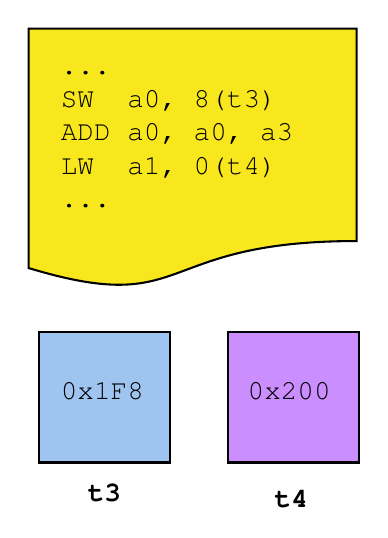
\begin{tikzpicture}[x=0.75pt,y=0.75pt,yscale=-1,xscale=1]
%uncomment if require: \path (0,263); %set diagram left start at 0, and has height of 263

%Flowchart: Document [id:dp9594301424377306] 
\draw  [fill={rgb, 255:red, 248; green, 231; blue, 28 }  ,fill opacity=1 ] (11,11) -- (169,11) -- (169,113.3) .. controls (70.25,113.3) and (90,150.19) .. (11,126.32) -- cycle ;
%Shape: Square [id:dp9762212690241732] 
\draw  [fill={rgb, 255:red, 74; green, 144; blue, 226 }  ,fill opacity=0.53 ] (16,157) -- (79,157) -- (79,220) -- (16,220) -- cycle ;
%Shape: Square [id:dp4447151686383942] 
\draw  [fill={rgb, 255:red, 144; green, 19; blue, 254 }  ,fill opacity=0.48 ] (107,157) -- (170,157) -- (170,220) -- (107,220) -- cycle ;

% Text Node
\draw (25,30) node [anchor=north west][inner sep=0.75pt]   [align=left] {{\fontfamily{pcr}\selectfont ...}\\{\fontfamily{pcr}\selectfont SW \ a0, 8(t3)}\\{\fontfamily{pcr}\selectfont ADD a0, a0, a3}\\{\fontfamily{pcr}\selectfont LW \ a1, 0(t4)}\\{\fontfamily{pcr}\selectfont ...}};
% Text Node
\draw (25,180) node [anchor=north west][inner sep=0.75pt]   [align=left] {{\fontfamily{pcr}\selectfont 0x1F8}};
% Text Node
\draw (38,229) node [anchor=north west][inner sep=0.75pt]   [align=left] {{\fontfamily{pcr}\selectfont \textbf{t3}}};
% Text Node
\draw (128,232) node [anchor=north west][inner sep=0.75pt]   [align=left] {{\fontfamily{pcr}\selectfont \textbf{t4}}};
% Text Node
\draw (115,180) node [anchor=north west][inner sep=0.75pt]   [align=left] {{\fontfamily{pcr}\selectfont 0x200}};


\end{tikzpicture}
\end{center}
	\label{fig:static-analysis-problem}
	\caption[The Limitations of Static Analysis]{This shows a programming code fragment of RISC-V assembly code and two registers \texttt{t3} and \texttt{t4}. Without conducting extensive simulation of all register accesses it would be impossible for a static analysis tool to know that at this point in the program \texttt{t3} and \texttt{t4} refer to the same memory address. Consequently re-ordering these instructions, though it might look safe could lead to the program not functioning as the programmer intended.}
\end{figure}

There has been very little work in online trace processing, i.e. processing and reacting to the trace while the program is running, and even less work on applying those ideas to the problem of latency reduction, which we'll explore in the conclusion and future sections. However some work has been done to utilise tracing in various offline processes, some of which are detailed in the next few sections. To bring this consideration of the literature to a close we'll also consider some examples of work done on using tracing as a method of on-chip debugging as this forms the basis for the implementation that will be presented in future chapters.

\subsection{Tracing as a Control Loop}

Tracing is most often used as a tool to generate large amounts of data that can be explored offline, with engineers then making manual adjustments to the program as a result of the knowledge gained from the trace. \citet{huApplicationsOnchipTrace2007} is an example of this with the TraceDo System. This system, aggregates traces from \glsplural{dsp} in the \gls{soc} and streams them into an emulator that adds timestamps to the various events. The data is then explored offline and is used to optimise long running functions in the program. \citet{wangRealTimeCache2013} make similar use of an emulator but utilise the trace to drive cache emulation in a separate process, continuing a trend of making information useful to the programmer by not to the system. This trend continues in \citet{liTracebasedAnalysisMethodology2016} and \citet{mertzPracticalFeasibilitySoftware2019} and in addition they both focus on trace collection and reducing the size of the traces collected rather than on acting on the information the traces give.

The problem with all of these ideas is that they are all considering trace analysis and action to be done offline rather than as part of the system itself. Some authors have tried to make this work however, \citet{singhResourceThroughputAware2016} describes a process of mapping applications to cores on a \gls{mpsoc} while the applications are running. This is a step towards the kind of closed loop feedback that would be of benefit but sadly the trace collection is done at design-time not run-time. In addition this model targets throughput rather than latency reduction, but there's no reason why the objective function used couldn't be re-purposed. \citet{shoukryProactiveSchedulingContent2014} propose a system for scheduling content delivery on mobile devices, attempting, via the analysis of usage patterns, to predict what content users will want and fetching it via WiFi rather than placing a large burden on Mobile Data Networks. Though this example is from an entirely separate field this approach is exactly the one we should aim to emulate. There are questions to be answered about how accurate their statistical modelling is but nevertheless this is an example of a tight feedback loop, using traces to predict activity to increase performance. 

\subsection{Tracing for In-Silicon Debugging}

To finish this short section on tracing we will consider the use of tracing as a method of in-silicon debugging. While the relevance of this may not be immediately apparent, many of these papers formed the basis for the implementation of the solution that will be presented in Chapters \ref{chap:trace-assisted-caching} and \ref{chap:experimental-design}. The first of these is \citet{uzelacHardwareBasedLoadValue2013} who present an off-chip debug host that mirrors the internals of the system being traced. This idea in turn is picked up by \citet{deckerOnlineAnalysisDebug2018} who also start to do the analysis in this offline module, converting the trace stream to series of events that can be processed. This idea, of taking a large amount of trace information and filtering the crucial events, while also having to deal with instruction reconstruction, is crucial for the development of our solution in Chapter \ref{chap:trace-assisted-caching}. A couple of ancillary issues are covered by other papers: \citet{scheipelSystemAwarePerformanceMonitoring2017} describe a method of tracking execution time in RISC-V processors without interfering with the system itself, but this is conceived as a set of performance counters on the chip. This is developed by \citet{delshadtehraniNileProgrammableMonitoring2018} who describe a programmable co-processor for tracking execution time which was crucial for the design of Gouram, which will be seen in Chapter \ref{chap:experimental-design}. 

\section{Conclusion}

Having considered a vast swathe of the literature in the last three sections we are forced to ask where this leaves us. Our goal of reducing latency appears to be blocked along the many paths we have considered. Solutions which attempt to improve the cache, via cache policy, are bounded above by \texttt{OPT}, which does not itself reduce misses to 0 due to compulsory misses and a finite cache capacity. Solutions that target the cache architecture are very well in their way, but do not address the basic problem that they are trying to make decisions with a paltry amount of information because of the need to decouple all these systems from each other. Certain papers propose integrating the cache and memory controllers, for example \cite{stuecheliCoordinatingDRAMLastLevelCache2011}, but there is not the integration across all components of the system, from the compiler to the memory hardware, that would give the information necessary to make better decisions.

Moving outside the cache, prefetching seems like a sensible way to solve these problems, and could be added on to almost any other solution but it's failures come down again to the lack of information available to the pre-fetching unit. As a result most pre-fetching comes down to recognising patterns or attempting to derive the future from the past which whilst good is not foolproof, especially as the diversity of application increases. Scheduling and program transformation also look promising but the inability to incorporate dynamic information limits their utility to what can be predicted statically which is a relatively small amount of information. 

\subsection{Potential for the application of Tracing}

So it would appear that there is little more that could be done, other than tinker at the edges with cache policies or pre-fetch units and hope that the processor-memory gap shrinks of its own accord. But what if there was a way to address the lack of information that is at the heart of the problems we've seen? What if we could fuse together pre-fetching and cache policy with dynamic information gathered from traces? Caches could act pre-emptively to fetch data they know will be required, utilising existing slack in programs to improve their overall runtime by better hiding the latency that exists. This is the basis of Trace-Assisted Caching which will be explored in much more detail in the next chapter. 

